\documentclass[margin=5mm]{standalone}
\usepackage[dvipsnames]{xcolor}
\usepackage{pgfplots}
\usepackage{tikz}
\usepackage[tikz]{ocgx2}

\pgfplotsset{compat=1.18}
\begin{document}

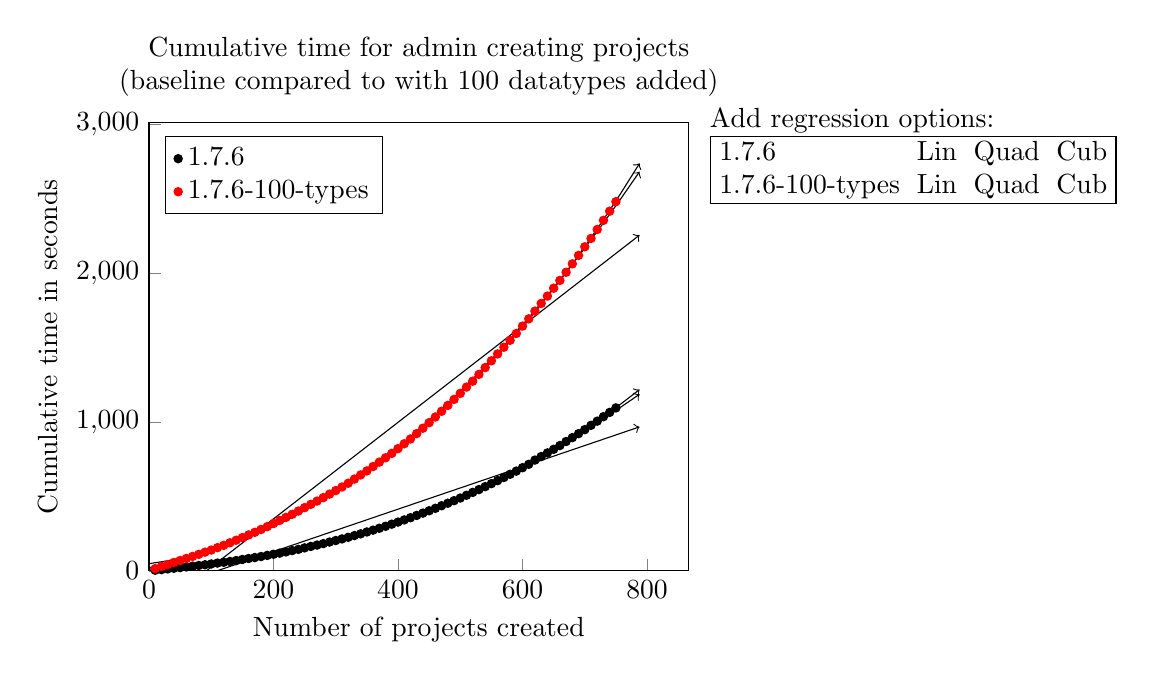
\begin{tikzpicture}
    \begin{axis}[
        align = center,
        legend pos = north west,
        legend cell align = left,
        xlabel = Number of projects created,
        ylabel = Cumulative time in seconds,
        xtick pos = left,
        ytick pos = left,
        scaled ticks = false,
        xmin = 0,
        ymin = 0,
        title = {Cumulative time for admin creating projects (baseline compared to with 100 datatypes added)},
        title style = {text width = 0.8\textwidth},
        legend entries={\switchocg{1.7.6}{1.7.6},\switchocg{1.7.6-100-types}{1.7.6-100-types}}]
        \begin{scope}[ocg = {ref = 1.7.6-Lin, status = invisible}]
            \plot[domain=0:788,->,forget plot] (\x,{-155.0244572972973173818900249898433685302734375 + 1.4244300455192036025664492626674473285675048828125*(\x)^1});
        \end{scope}
        \begin{scope}[ocg = {ref = 1.7.6-Quad, status = invisible}]
            \plot[domain=0:788,->,forget plot] (\x,{23.504802310255247022041658055968582630157470703125 + 0.033292957668144086691430771907107555307447910308837890625*(\x)^1 + 0.00183044353664613156963680840050301412702538073062896728515625*(\x)^2});
        \end{scope}
        \begin{scope}[ocg = {ref = 1.7.6-Cub, status = invisible}]
            \plot[domain=0:788,->,forget plot] (\x,{2.016385233452537395493209260166622698307037353515625 + 0.3617561252642944591428886269568465650081634521484375*(\x)^1 + 0.0007570960303123239025502311250193088199011981487274169921875*(\x)^2 + 0.0000009415329002928142330743912190305078269147998071275651454925537109375*(\x)^3});
        \end{scope}
        \begin{scope}[ocg = {ref = 1.7.6, status = visible}]
            \addplot[
                only marks,
                color = black,
                mark = *,
                mark size = 1.5 pt
            ]coordinates {(10,4.557)(20,8.772)(30,13.693)(40,18.002)(50,22.472)(60,27.02)(70,31.771)(80,36.649)(90,41.438)(100,46.874)(110,52.878)(120,58.273)(130,63.685)(140,69.652)(150,77.036)(160,83.559)(170,89.895)(180,96.757)(190,104.601)(200,112.046)(210,119.688)(220,127.754)(230,136.629)(240,145.014)(250,154.969)(260,164.572)(270,173.861)(280,183.438)(290,194.028)(300,204.25)(310,214.934)(320,225.971)(330,237.303)(340,249.061)(350,261.571)(360,273.836)(370,286.665)(380,299.845)(390,313.982)(400,328.075)(410,342.655)(420,357.416)(430,372.908)(440,388.373)(450,404.098)(460,420.486)(470,437.834)(480,454.759)(490,471.803)(500,489.623)(510,508.167)(520,527.486)(530,546.255)(540,566.059)(550,586.194)(560,606.424)(570,627.414)(580,648.792)(590,670.391)(600,693.259)(610,716.064)(620,744.494)(630,768.226)(640,792.551)(650,816.916)(660,841.934)(670,869.071)(680,895.131)(690,921.827)(700,948.878)(710,977.709)(720,1005.894)(730,1035.777)(740,1064.732)(750,1094.746)};
        \end{scope}
        \begin{scope}[ocg = {ref = 1.7.6-100-types-Lin, status = invisible}]
            \plot[domain=0:788,->,forget plot] (\x,{-298.46982846846884740443783812224864959716796875 + 3.240687513513514250718117182259447872638702392578125*(\x)^1});
        \end{scope}
        \begin{scope}[ocg = {ref = 1.7.6-100-types-Quad, status = invisible}]
            \plot[domain=0:788,->,forget plot] (\x,{48.70917246945490575171788805164396762847900390625 + 0.53539659711410758635707907160394825041294097900390625*(\x)^1 + 0.003559593311051851595439021735955975600518286228179931640625*(\x)^2});
        \end{scope}
        \begin{scope}[ocg = {ref = 1.7.6-100-types-Cub, status = invisible}]
            \plot[domain=0:788,->,forget plot] (\x,{10.6814186449455430505395270301960408687591552734375 + 1.1166733115934175391004146149498410522937774658203125*(\x)^1 + 0.00166010510802939471874939414419714012183248996734619140625*(\x)^2 + 0.000001666217721949524402272162226790186423386330716311931610107421875*(\x)^3});
        \end{scope}
        \begin{scope}[ocg = {ref = 1.7.6-100-types, status = visible}]
            \addplot[
                only marks,
                color = red,
                mark = *,
                mark size = 1.5 pt
            ]coordinates {(10,15.817)(20,30.289)(30,42.729)(40,56.998)(50,70.189)(60,83.756)(70,97.381)(80,111.429)(90,126.099)(100,140.278)(110,156.394)(120,171.907)(130,189.128)(140,206.196)(150,223.852)(160,241.619)(170,259.505)(180,278.492)(190,297.584)(200,318.088)(210,339.682)(220,359.566)(230,380.439)(240,402.47)(250,425.076)(260,447.36)(270,469.269)(280,492.256)(290,515.683)(300,539.641)(310,563.692)(320,588.874)(330,616.926)(340,644.586)(350,671.694)(360,701.301)(370,730.817)(380,759.857)(390,789.45)(400,821.31)(410,853.973)(420,886.138)(430,922.249)(440,958.575)(450,995.661)(460,1033.862)(470,1072.337)(480,1111.566)(490,1151.63)(500,1192.36)(510,1234.479)(520,1274.251)(530,1319.789)(540,1365.486)(550,1411.136)(560,1457.212)(570,1502.171)(580,1548.484)(590,1594.435)(600,1644.134)(610,1692.578)(620,1744.681)(630,1796.486)(640,1845.709)(650,1898.643)(660,1950.902)(670,2005.624)(680,2061.977)(690,2118.775)(700,2176.416)(710,2232.481)(720,2292.876)(730,2354.245)(740,2415.768)(750,2479.589)};
        \end{scope}
    \end{axis}
    \begin{scope}
        \addtolength{\tabcolsep}{-0.3em}
        \node [below right, shape=rectangle, align=left](regressiontable) at (7,6) {
            Add regression options: \\
            \begin{tabular}{|llll|}
                \hline
                1.7.6 & \switchocg{1.7.6-Lin}{Lin} & \switchocg{1.7.6-Quad}{Quad} & \switchocg{1.7.6-Cub}{Cub} \\
                1.7.6-100-types & \switchocg{1.7.6-100-types-Lin}{Lin} & \switchocg{1.7.6-100-types-Quad}{Quad} & \switchocg{1.7.6-100-types-Cub}{Cub} \\
                \hline
            \end{tabular}
        };
    \end{scope}
\end{tikzpicture}

\end{document}